\documentclass[12pt,a4paper]{article}

\usepackage[spanish,es-nodecimaldot]{babel}
\usepackage[T1]{fontenc}
\usepackage[utf8]{inputenc}
\usepackage{lmodern}
\usepackage[a4paper,margin=2.5cm]{geometry}
\usepackage{setspace}
\usepackage{parskip}
\usepackage{booktabs}
\usepackage{tabularx}
\usepackage{array}
\usepackage{ragged2e}
\usepackage{xcolor}
\usepackage{hyperref}
\usepackage{enumitem}
\usepackage{graphicx}
\usepackage{tikz}

\usetikzlibrary{arrows.meta,positioning,shapes.geometric}

\hypersetup{
  colorlinks=true,
  linkcolor=black,
  urlcolor=blue!60!black,
  citecolor=black
}

\definecolor{cibblue}{HTML}{0F4C81}
\definecolor{cibteal}{HTML}{1F7A8C}

\tikzset{
  box/.style={draw=cibblue, rounded corners, fill=cibblue!8, minimum width=2.2cm, minimum height=0.95cm, align=center, font=\small},
  smallbox/.style={draw=cibteal, rounded corners, fill=cibteal!8, minimum width=2.0cm, minimum height=0.85cm, align=center, font=\small},
  line/.style={-{Latex[length=2mm]}, thick, draw=cibblue}
}

\setstretch{1.15}
\setlist[itemize]{itemsep=0.25em, topsep=0.4em}
\setlist[enumerate]{itemsep=0.25em, topsep=0.4em}

\title{\textbf{Procesamiento de Flujos de Datos en Tiempo Real a Gran Escala}\\[0.4em]
\large Monografia basada en el capitulo 4 de \textit{huawei-2022.pdf}}
\author{Curso CIB12 - Aprendizaje de Maquina y Mineria de Datos\\Grupo 6}
\date{2026}

\begin{document}

\hypersetup{pageanchor=false}
\begin{titlepage}
  \centering
  \vspace*{0.8cm}
  {\large \textbf{Universidad Nacional de Ingeniería}\par}
  \vspace{0.35cm}
  {\large \textbf{Facultad de Ingeniería Eléctrica y Electrónica}\par}
  \vspace{0.8cm}
  
\includegraphics[width=3.1cm]{uni.png}\par
  \vspace{0.8cm}
  {\Large \textbf{Aprendizaje de Máquina y Minería de Datos}\par}
  \vspace{0.9cm}
  {\Large \textbf{Procesamiento de Flujos de Datos en}\par}
  {\Large \textbf{Tiempo Real a Gran Escala}\par}
  \vspace{0.35cm}
  {\normalsize Monografía basada en el capítulo 4 de \textit{huawei-2022.pdf}\par}
  \vspace{1cm}
  {\large \textbf{GRUPO 6}\par}
  \vspace{0.5cm}
  {\normalsize \textbf{Integrantes:}\par}
  \vspace{0.3cm}
  {\normalsize Jhunior Eduardo Guevara Lázaro\par}
  \vspace{0.7cm}
  {\normalsize \textbf{Docente:}\par}
  \vspace{0.3cm}
  {\normalsize Mg. Ing. Yury Tello Canchapoma\par}
  \vfill
  {\large \textbf{LIMA - PERÚ}\par}
  \vspace{0.25cm}
  {\large \textbf{2026}\par}
\end{titlepage}
\hypersetup{pageanchor=true}

\pagenumbering{roman}
\setcounter{page}{1}

\section*{Resumen}
\addcontentsline{toc}{section}{Resumen}

\begin{abstract}
El procesamiento de flujos de datos en tiempo real se ha convertido en una capacidad central para sistemas modernos que necesitan reaccionar ante eventos antes de que su valor se degrade. El capitulo 4 del material \textit{HCIP Big Data Developer V2.0 Training Material} de Huawei presenta una vision aplicada de este problema, su arquitectura de referencia y un conjunto de tecnologias clave para ingesta, mensajeria, computo distribuido y respuesta de baja latencia. La presente monografia sintetiza y amplía ese contenido con el objetivo de explicar los fundamentos del \textit{stream processing}, comparar sus principales componentes tecnologicos y relacionarlos con casos de uso reales como deteccion de fraude, analitica de comercio electronico, monitoreo IoT y ciberseguridad. Asimismo, se incorporan conceptos tecnicos imprescindibles para la construccion de un laboratorio, tales como tiempo de evento, ventanas, estado, \textit{checkpoints}, \textit{watermarks} y semanticas de entrega. El resultado es una base conceptual y aplicada para el desarrollo de una presentacion academica y de una implementacion practica orientada al curso.
\end{abstract}

\newpage
\tableofcontents
\newpage
\pagenumbering{arabic}
\setcounter{page}{1}

\section{Introduccion}

El crecimiento del volumen, velocidad y diversidad de los datos ha impulsado el desarrollo de arquitecturas capaces de procesar informacion mientras esta se encuentra en movimiento. En muchos escenarios, esperar a que los datos sean almacenados para analizarlos mas tarde ya no es suficiente. Una transaccion fraudulenta, una anomalia en una linea de produccion o una recomendacion comercial pierden valor si la respuesta llega tarde.

En este contexto, el procesamiento de flujos de datos en tiempo real busca transformar eventos continuos en decisiones operativas con baja latencia. El capitulo 4 del libro base estudia precisamente este problema y propone una solucion articulada alrededor de tecnologias como Flume, Kafka, Flink, Structured Streaming y Redis. Su aporte principal es mostrar que el valor del dato no es constante en el tiempo, y que por ello la velocidad de analisis se convierte en una variable de negocio.

La presente monografia tiene tres objetivos. Primero, explicar con claridad el problema que resuelve el procesamiento en tiempo real y diferenciarlo del procesamiento \textit{batch}. Segundo, describir la arquitectura y las tecnologias que permiten construir una plataforma de \textit{stream processing} a gran escala. Tercero, conectar estos conceptos con casos de uso y con una futura implementacion en codigo para laboratorio.

\section{Procesamiento en Tiempo Real en Big Data}

\subsection{Problema y motivacion}

El capitulo 4 plantea que algunos datos tienen valor maximo inmediatamente despues de que ocurre el evento que los genera. Si una plataforma tarda minutos u horas en analizarlos, la oportunidad de actuar puede perderse. Por ello, la meta del procesamiento en tiempo real no es solamente almacenar informacion, sino convertirla en accion mientras el evento sigue siendo relevante.

Este enfoque es especialmente importante en escenarios como los siguientes:

\begin{itemize}
  \item deteccion de fraude financiero;
  \item monitoreo de infraestructura y servicios;
  \item analitica operacional en comercio electronico;
  \item sistemas IoT y mantenimiento predictivo;
  \item ciberseguridad y correlacion de eventos.
\end{itemize}

\subsection{Diferencia entre batch, retrieval y stream processing}

El procesamiento \textit{batch} se orienta al analisis de datos historicos acumulados. Su fortaleza es el calculo exhaustivo sobre grandes volumenes, aunque con alta tolerancia a la latencia. En contraste, el \textit{real-time retrieval} prioriza recuperar datos ya almacenados con tiempos de respuesta muy bajos, por ejemplo mediante sistemas en memoria o motores de consulta rapida.

El \textit{stream processing}, en cambio, trabaja sobre datos en movimiento. No espera a que el conjunto de datos este completo, sino que procesa cada evento a medida que llega. Esto implica un modelo de computo continuo, con manejo de estado, tolerancia a fallos y mecanismos para trabajar con eventos fuera de orden.

\begin{figure}[h]
\centering
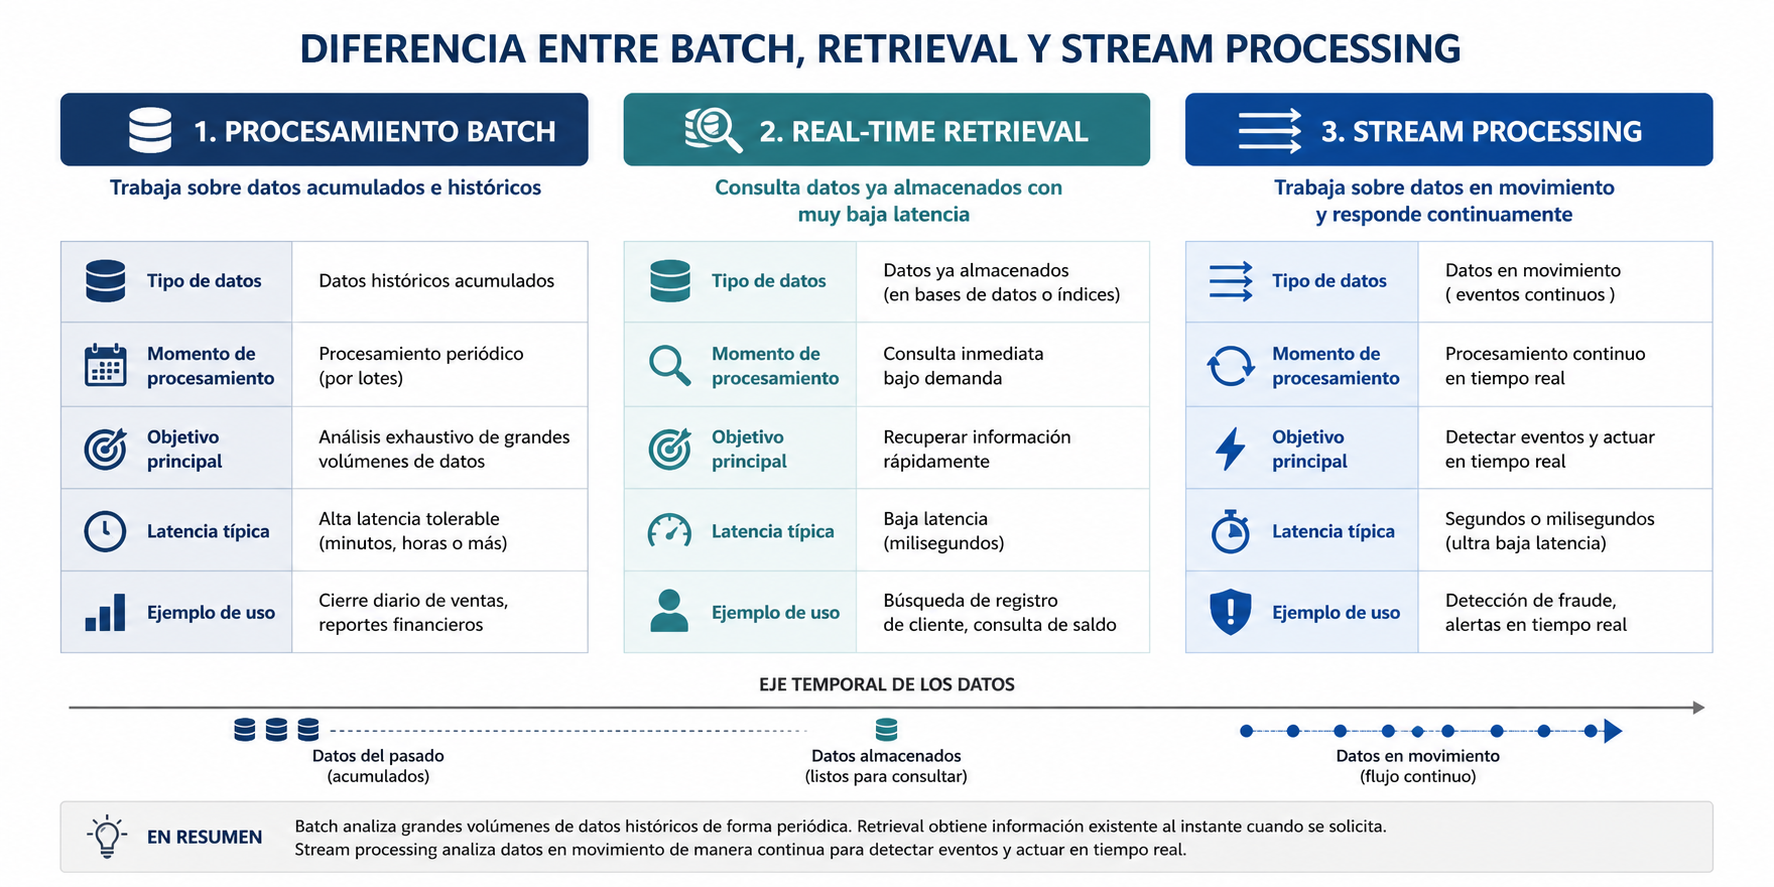
\includegraphics[width=\textwidth]{img/01.png}
\caption{Comparacion entre procesamiento batch, \textit{real-time retrieval} y \textit{stream processing}}
\label{fig:batch-retrieval-stream}
\end{figure}





\subsection{Requisitos de una plataforma a gran escala}

Una solucion de procesamiento en tiempo real a gran escala debe cumplir al menos con los requisitos de la Tabla~\ref{tab:requisitos}.

\begin{table}[h]
\centering
\caption{Requisitos principales de una plataforma de \textit{stream processing}}
\label{tab:requisitos}
\begin{tabularx}{\textwidth}{>{\RaggedRight\arraybackslash}p{4cm}X}
\toprule
\textbf{Requisito} & \textbf{Descripcion} \\
\midrule
Baja latencia & Procesamiento en segundos o milisegundos para que el dato siga teniendo valor operativo. \\
Alto throughput & Capacidad de absorber y procesar miles o millones de eventos por segundo. \\
Alta confiabilidad & Evitar perdida de datos, duplicacion no controlada y fallos silenciosos. \\
Escalabilidad horizontal & Incrementar capacidad agregando nodos al cluster. \\
Multiples fuentes & Integrarse con logs, bases de datos, archivos, sensores, APIs y mensajeria. \\
Aislamiento y control & Separar recursos, cargas y permisos entre usuarios o aplicaciones. \\
Integracion externa & Conectarse con motores de reglas, dashboards, caches y sistemas transaccionales. \\
\bottomrule
\end{tabularx}
\end{table}

\section{Marco Conceptual}

\subsection{Flujos, eventos y procesamiento continuo}

Un flujo de datos es una secuencia continua de eventos generados a lo largo del tiempo. Un evento representa una ocurrencia concreta, por ejemplo una compra, un clic, una lectura de sensor o una solicitud HTTP. Cada evento contiene atributos y, normalmente, una marca temporal.

Procesar un flujo implica aplicar transformaciones, filtros, agregaciones o modelos a esos eventos conforme van llegando. Esto obliga a considerar el tiempo como una dimension de primer orden. A diferencia de un conjunto estatico de datos, el flujo nunca esta completamente cerrado, por lo que el sistema debe decidir continuamente cuando emitir resultados parciales o finales.

Desde una perspectiva de sistemas, el procesamiento continuo cambia la logica tradicional del analisis de datos. En un entorno \textit{batch}, el sistema espera a tener un conjunto de datos delimitado y luego ejecuta una tarea completa. En cambio, en \textit{stream processing} el computo se mantiene activo y reacciona a cada nuevo evento. Por ello, conceptos como orden temporal, consistencia incremental y recuperacion del estado pasan a ser tan importantes como el algoritmo de negocio.

\subsection{Tiempo de evento y tiempo de procesamiento}

Dos referencias temporales son fundamentales:

\begin{itemize}
  \item \textbf{Tiempo de evento}: instante en que el hecho ocurrio en la fuente.
  \item \textbf{Tiempo de procesamiento}: instante en que el sistema recibe o procesa el evento.
\end{itemize}

Si una red introduce retrasos o si la fuente envia datos de manera irregular, estas dos nociones pueden diferir significativamente. Para analitica precisa, suele preferirse el tiempo de evento, ya que representa mejor el orden real de los sucesos. La investigacion tambien resalta una tercera nocion, el \textit{tiempo de ingestión}, que corresponde al instante en que el evento entra al broker o al sistema de streaming. Esta referencia puede ser util cuando el origen no provee marcas temporales confiables, aunque sigue siendo menos precisa que el tiempo de evento para reconstruir lo que realmente ocurrio en el dominio del problema.

La eleccion entre estas nociones temporales tiene consecuencias practicas. Usar tiempo de procesamiento simplifica la implementacion, pero puede distorsionar los resultados cuando hay retrasos, reintentos o llegadas fuera de orden. Usar tiempo de evento introduce mayor complejidad, aunque permite calculos mas fieles en escenarios como fraude, IoT o analitica de usuarios.

\begin{figure}[h]
\centering
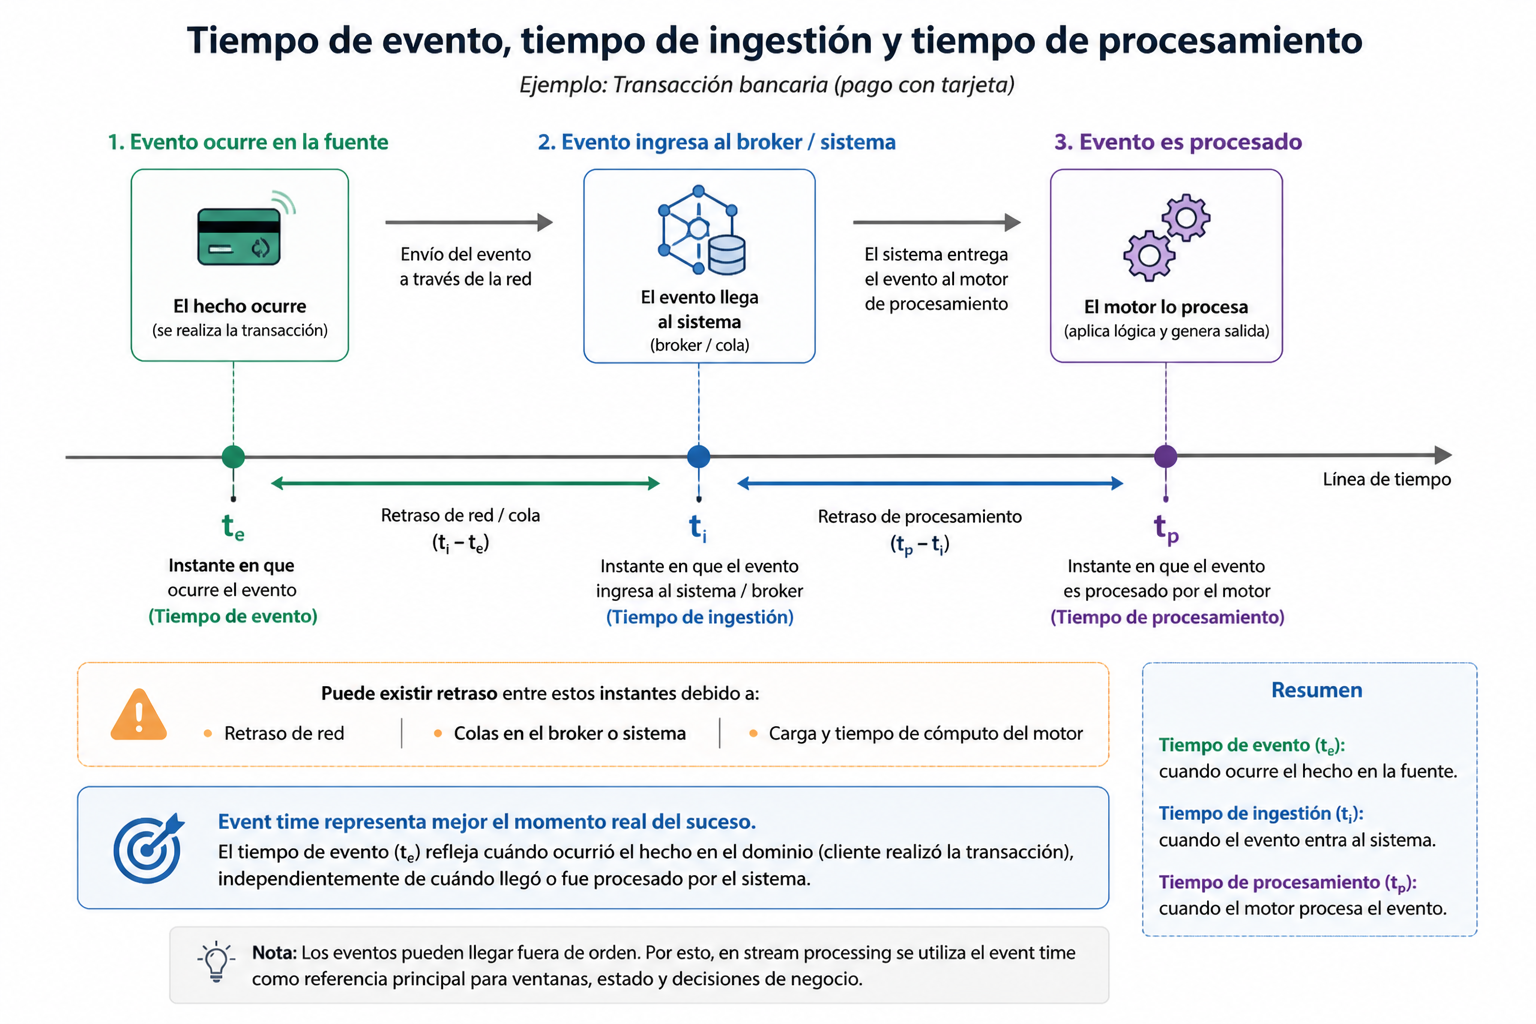
\includegraphics[width=\textwidth]{img/02.png}
\caption{Relacion entre tiempo de evento, tiempo de ingestión y tiempo de procesamiento}
\label{fig:event-ingestion-processing-time}
\end{figure}

\subsection{Ventanas temporales}

Como un flujo no tiene fin definido, las agregaciones necesitan limitarse mediante ventanas. Las mas comunes son:

\begin{itemize}
  \item \textbf{Tumbling windows}: intervalos fijos sin solapamiento.
  \item \textbf{Sliding windows}: intervalos fijos con solapamiento.
  \item \textbf{Session windows}: intervalos definidos por periodos de inactividad.
\end{itemize}

Las ventanas permiten responder preguntas como cuantas compras ocurrieron en los ultimos diez minutos, cual fue el monto total por usuario durante una sesion o que productos fueron los mas vendidos en una franja temporal. La investigacion tambien menciona la utilidad de ventanas instantaneas o agregaciones puntuales sobre marcas de tiempo especificas, asi como la diferencia entre ventanas basadas en tiempo y ventanas basadas en conteo. Esta distincion es importante porque no todas las aplicaciones agrupan por minutos u horas; algunas necesitan cerrar la agregacion cuando se acumula un numero determinado de eventos.

En la practica, las ventanas no solo agrupan datos: tambien determinan cuando un resultado se considera suficientemente estable para ser emitido. Por eso estan estrechamente relacionadas con los \textit{watermarks} y con el tratamiento de eventos tardios.

\begin{figure}[h]
\centering
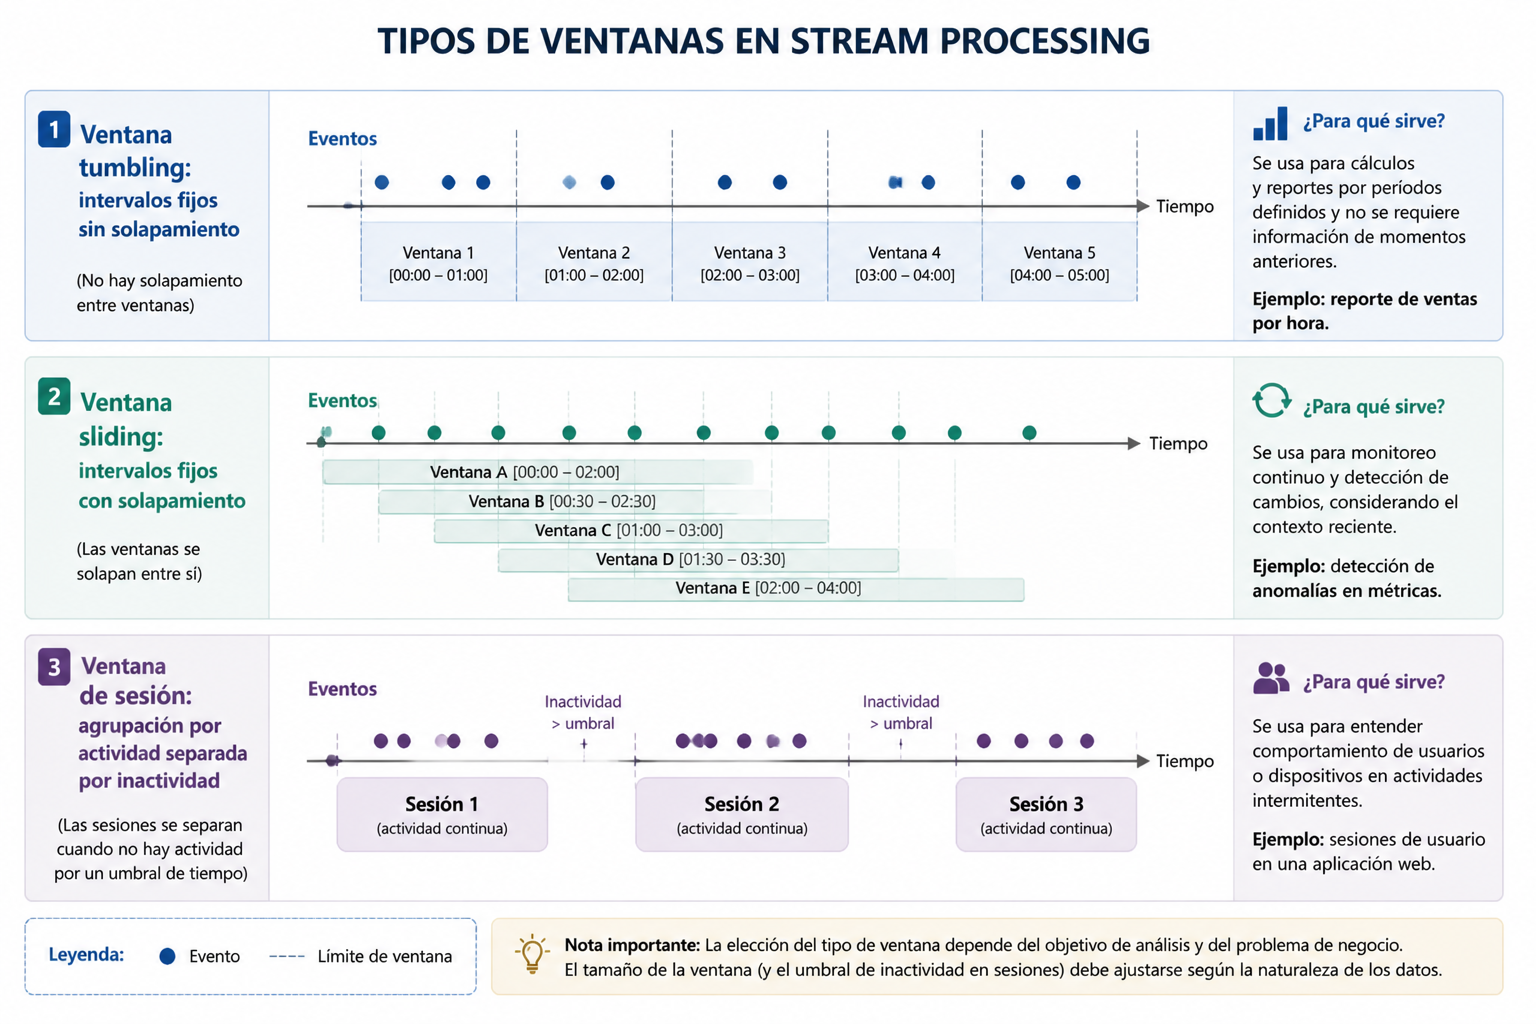
\includegraphics[width=\textwidth]{img/03.png}
\caption{Tipos principales de ventanas en procesamiento de streams}
\label{fig:stream-windows}
\end{figure}

\subsection{Estado, checkpoints y tolerancia a fallos}

Muchas operaciones de \textit{stream processing} son \textit{stateful}, es decir, dependen de informacion acumulada. Un contador por usuario, una suma parcial por ventana o una tabla intermedia de correlacion son ejemplos de estado.

Para evitar perder consistencia ante fallos, los motores de procesamiento registran \textit{checkpoints}: instantaneas periodicas del estado global y de la posicion de lectura en las fuentes. Si ocurre una caida, el job puede restaurarse desde el ultimo punto consistente.

En Flink, por ejemplo, la tolerancia a fallos se apoya en el uso de barreras de checkpoint que recorren el flujo y permiten construir un \textit{snapshot} consistente del grafo de operadores. Este mecanismo resulta esencial en aplicaciones de larga duracion, donde reiniciar desde cero no es viable. Gracias a ello, el procesamiento puede continuar despues de una falla sin perder totalmente el trabajo previo ni comprometer la consistencia del resultado.

\begin{figure}[h]
\centering
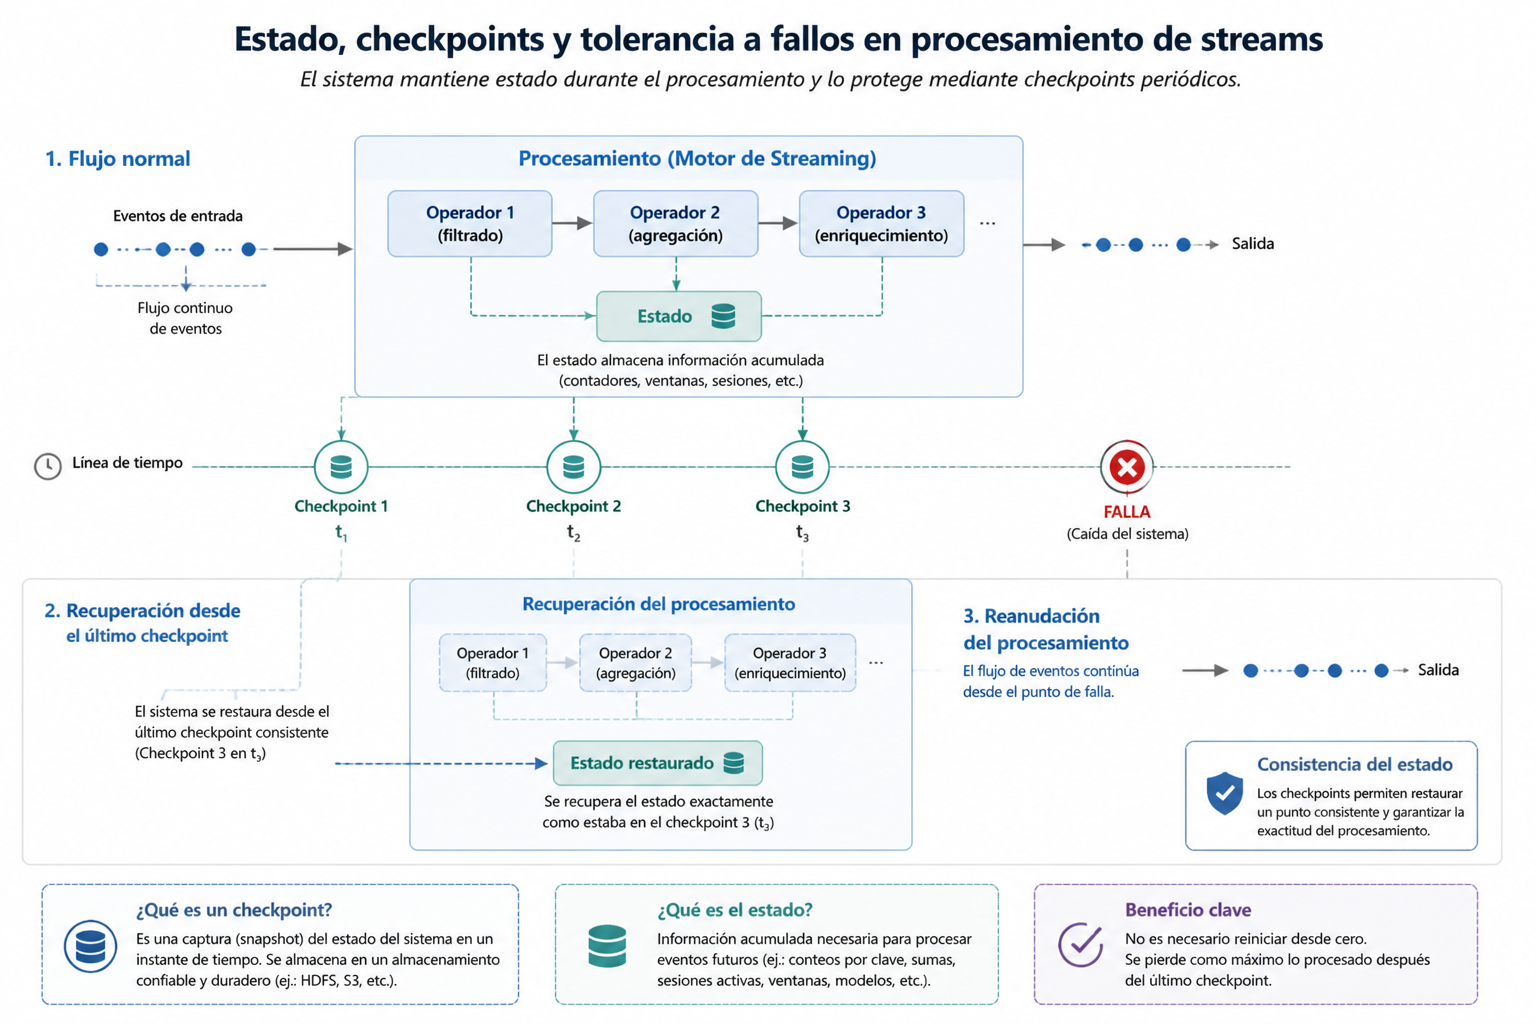
\includegraphics[width=\textwidth]{img/04.png}
\caption{Estado, checkpoints y recuperacion ante fallos en un sistema de procesamiento de streams}
\label{fig:state-checkpoints-recovery}
\end{figure}

\subsection{Eventos tardios, watermarks y semanticas de entrega}

En sistemas reales, los eventos no siempre llegan en el orden en que ocurrieron. Para manejar esta situacion se utilizan \textit{watermarks}, marcas que indican hasta que instante se considera razonable esperar eventos de tiempo anterior. Gracias a ello, el sistema puede cerrar ventanas aun cuando exista cierto desorden. En terminos practicos, un \textit{watermark} declara que hasta cierto punto ya se recibio toda la informacion relevante, lo que permite emitir resultados sin esperar indefinidamente.

Adicionalmente, un pipeline de streaming debe definir sus garantias de entrega:

\begin{itemize}
  \item \textbf{At-least-once}: un evento se procesa al menos una vez, con posibilidad de duplicados.
  \item \textbf{Exactly-once}: cada evento impacta el resultado una sola vez desde la perspectiva observable.
\end{itemize}

La segunda garantia es mas exigente y suele requerir coordinacion entre la fuente, el motor de procesamiento y el \textit{sink}. Cuando no es viable, una estrategia comun es usar \textit{sinks} idempotentes, es decir, destinos donde repetir la misma operacion no altere el resultado final. Esta idea es especialmente relevante cuando se trabaja con micro-batches, reprocesamientos o reinicios por falla.

\begin{figure}[h]
\centering
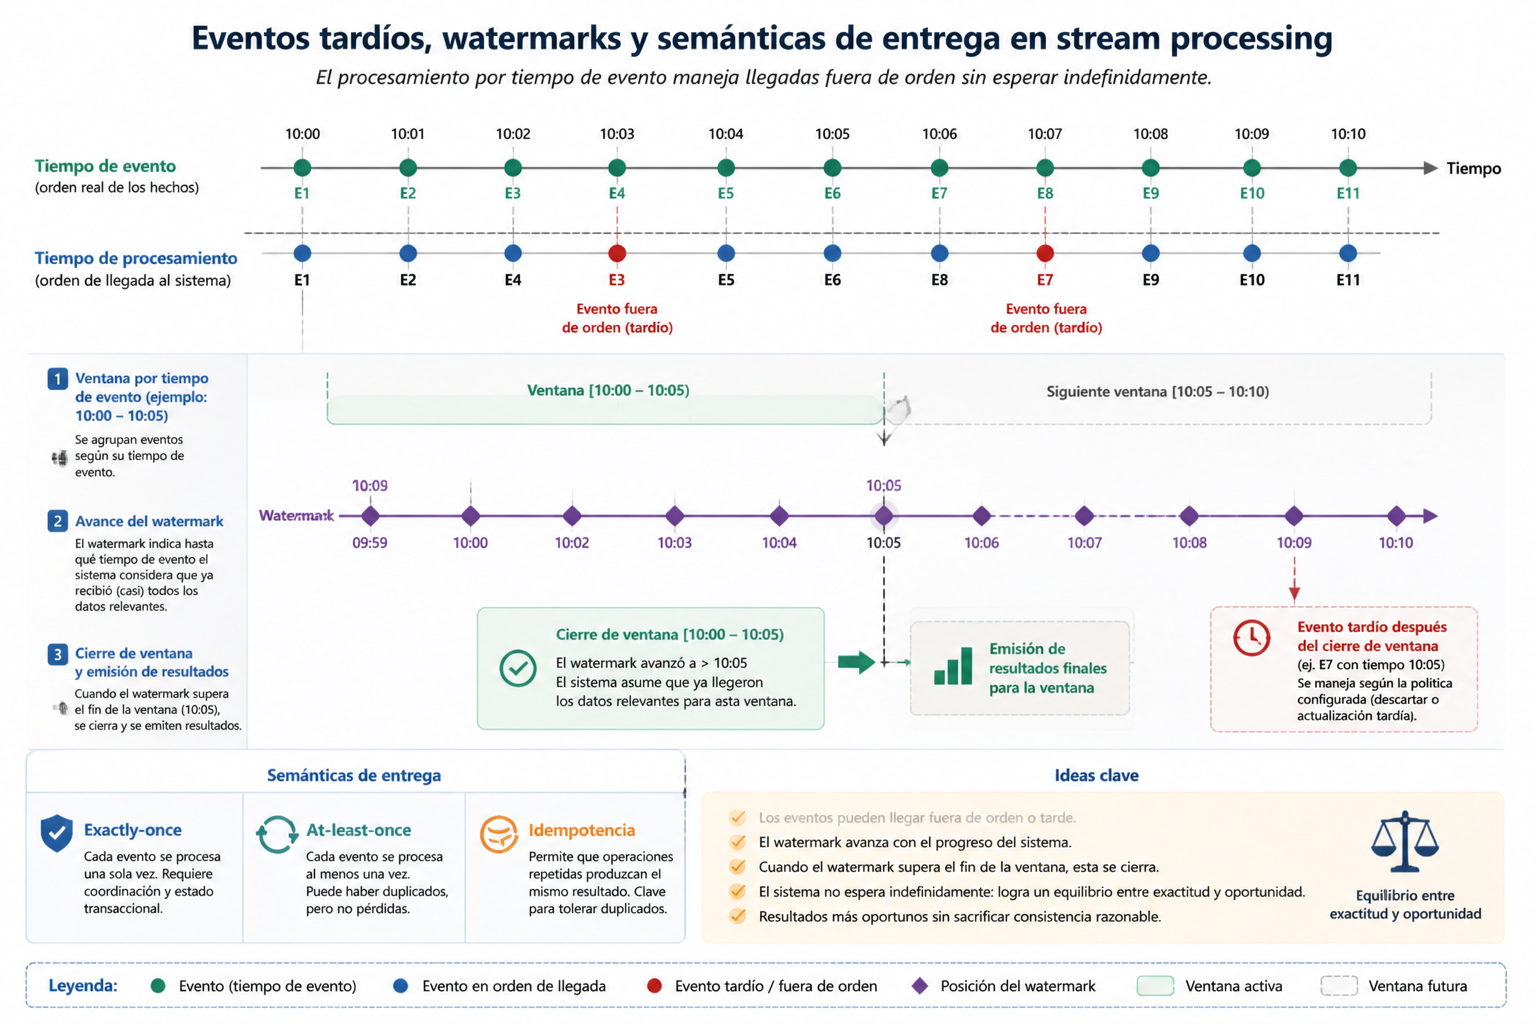
\includegraphics[width=\textwidth]{img/05.png}
\caption{Eventos tardios y uso de \textit{watermarks} para decidir el cierre de ventanas}
\label{fig:late-events-watermarks}
\end{figure}

En conjunto, el marco conceptual del streaming muestra que el problema no consiste solo en mover datos rapido, sino en producir resultados correctos, temporales y recuperables sobre una corriente de eventos potencialmente infinita.

\section{Arquitectura de Referencia}

La arquitectura presentada en el capitulo puede resumirse como un pipeline continuo de cinco etapas: generacion de datos, recoleccion, cola o almacenamiento temporal, computo en tiempo real y salida operativa o analitica. La Figura~\ref{fig:pipeline} sintetiza este flujo.

\begin{figure}[h]
\centering
\begin{tikzpicture}[node distance=0.8cm]
  \node[box] (src) {Fuentes de\\datos};
  \node[box, right=of src] (ing) {Ingesta y\\recoleccion};
  \node[box, right=of ing] (bus) {Broker o cola\\de mensajes};
  \node[box, right=of bus] (proc) {Procesamiento\\en tiempo real};
  \node[box, right=of proc] (out) {Accion, cache\\o visualizacion};

  \draw[line] (src) -- (ing);
  \draw[line] (ing) -- (bus);
  \draw[line] (bus) -- (proc);
  \draw[line] (proc) -- (out);
\end{tikzpicture}
\caption{Pipeline general de procesamiento de flujos en tiempo real}
\label{fig:pipeline}
\end{figure}

Este enfoque desacopla los componentes. Las fuentes generan eventos; la capa de ingesta los normaliza o transporta; el broker absorbe picos y distribuye la carga; el motor de procesamiento ejecuta reglas, agregaciones o modelos; y finalmente los resultados se almacenan, visualizan o convierten en decisiones operativas.

La investigacion realizada muestra que esta arquitectura puede entenderse como una solucion extremo a extremo con cinco capas funcionales: fuentes, ingesta, procesamiento, almacenamiento y accion. Su fortaleza principal es la separacion de responsabilidades. Cada capa puede escalar independientemente y puede reemplazarse por otra tecnologia equivalente sin rehacer por completo el sistema.

\begin{figure}[h]
\centering
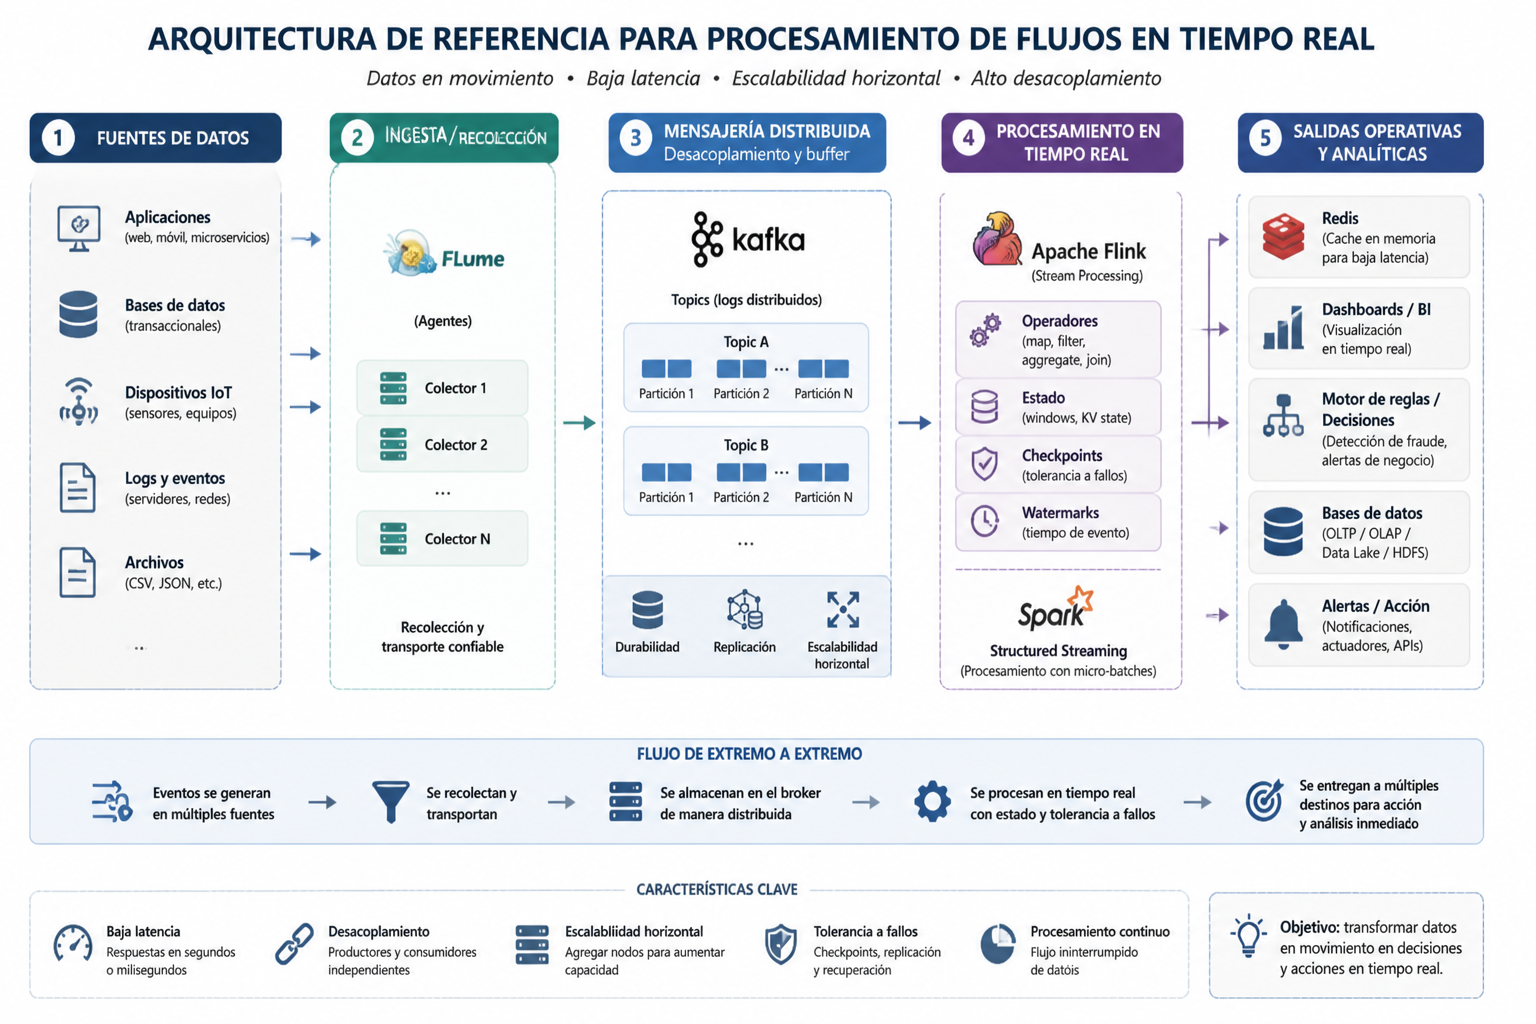
\includegraphics[width=\textwidth]{img/06.png}
\caption{Arquitectura de referencia detallada para procesamiento de flujos en tiempo real}
\label{fig:reference-architecture-detailed}
\end{figure}

\subsection{Fuentes y capa de ingesta}

Las fuentes pueden ser bases de datos, logs de aplicacion, sensores IoT, servicios web, archivos incrementales o plataformas externas. La ingesta tiene como finalidad recoger estos datos de forma confiable y entregarlos al resto del pipeline. En este nivel, el capitulo resalta a Flume como tecnologia de recoleccion.

La capa de ingesta cumple dos tareas complementarias. Primero, conecta con origenes heterogeneos y transforma datos brutos en eventos que el sistema pueda transportar. Segundo, aisla a las fuentes del resto de la arquitectura, de modo que los productores no dependan directamente de la logica de analisis. Esta separacion es importante cuando las fuentes son numerosas, poco confiables o generan picos abruptos de informacion.

\subsection{Broker de eventos}

El broker actua como una capa de desacoplamiento entre productores y consumidores. Su funcion es absorber picos, ordenar mensajes dentro de particiones, permitir consumo paralelo y ofrecer persistencia temporal. En la arquitectura del capitulo, Kafka cumple este rol.

Desde el punto de vista de diseno, el broker convierte un flujo dificil de controlar en un log distribuido que varios consumidores pueden leer a distinto ritmo. Esto permite que un mismo conjunto de eventos alimente simultaneamente analitica en tiempo real, dashboards, almacenamiento historico o motores de recomendacion. Ademas, facilita el reprocesamiento cuando una aplicacion necesita recomputar resultados a partir de eventos ya almacenados.

\subsection{Procesamiento y salida}

Sobre el broker se ubican motores como Flink o Structured Streaming, encargados de ejecutar logica de negocio, agregaciones por ventana, enriquecimiento de datos y deteccion de patrones. Finalmente, los resultados pueden enviarse a Redis, bases de datos, dashboards, motores de reglas o sistemas transaccionales.

La investigacion tambien subraya que la salida no siempre debe entenderse como almacenamiento final. En muchos casos, la meta es habilitar una accion inmediata: bloquear una transaccion, actualizar una recomendacion, disparar una alerta o alimentar una interfaz de monitoreo. Por ello, la arquitectura de referencia no termina en el computo, sino en la capacidad efectiva de transformar datos en respuesta operativa.

\subsection{Integracion extremo a extremo}

Un ejemplo integrador ayuda a entender la arquitectura completa. En un escenario de fraude bancario, las transacciones pueden originarse en canales de pago, ser recolectadas por agentes de ingesta, transportadas a Kafka, procesadas por Flink mediante ventanas y estado, y finalmente publicadas en Redis o en un sistema transaccional para ejecutar bloqueos o validaciones adicionales. En un escenario de e-commerce, la misma arquitectura puede cambiar la logica de negocio, pero no su estructura general: eventos de navegacion, ingestion, broker, procesamiento y salida hacia dashboards o motores de recomendacion.

Esta capacidad de reutilizar el mismo esqueleto arquitectonico en problemas distintos es una de las razones por las que el procesamiento de flujos se ha vuelto central en plataformas modernas de datos.

\section{Tecnologias Principales del Capitulo}

\subsection{Flume}

Flume es una herramienta de recoleccion distribuida de datos, especialmente orientada a logs y eventos. Su arquitectura clasica se basa en tres componentes: \textit{Source}, \textit{Channel} y \textit{Sink}. El \textit{Source} recibe eventos, el \textit{Channel} actua como buffer temporal y el \textit{Sink} envia la informacion al siguiente destino.

Entre sus ventajas destacan la simplicidad de despliegue, la recoleccion distribuida y la posibilidad de enriquecer o enrutar eventos mediante interceptores y selectores. La investigacion recupera ademas varias capacidades del capitulo: recoleccion desde directorios fijos o en seguimiento continuo, soporte para cascadas de multiples agentes, replicacion a varios destinos y configuraciones avanzadas mediante interceptores, selectores de canal y procesadores de \textit{sink}.

Tambien es importante notar que Flume no se limita a una estructura minima. Puede trabajar con distintos tipos de \textit{source}, \textit{channel} y \textit{sink}, incluyendo recepcion por HTTP, syslog, directorios, Kafka y HDFS. Su limitacion principal es que no esta pensado para analitica compleja, sino para ingesta y transporte.

\begin{figure}[h]
\centering
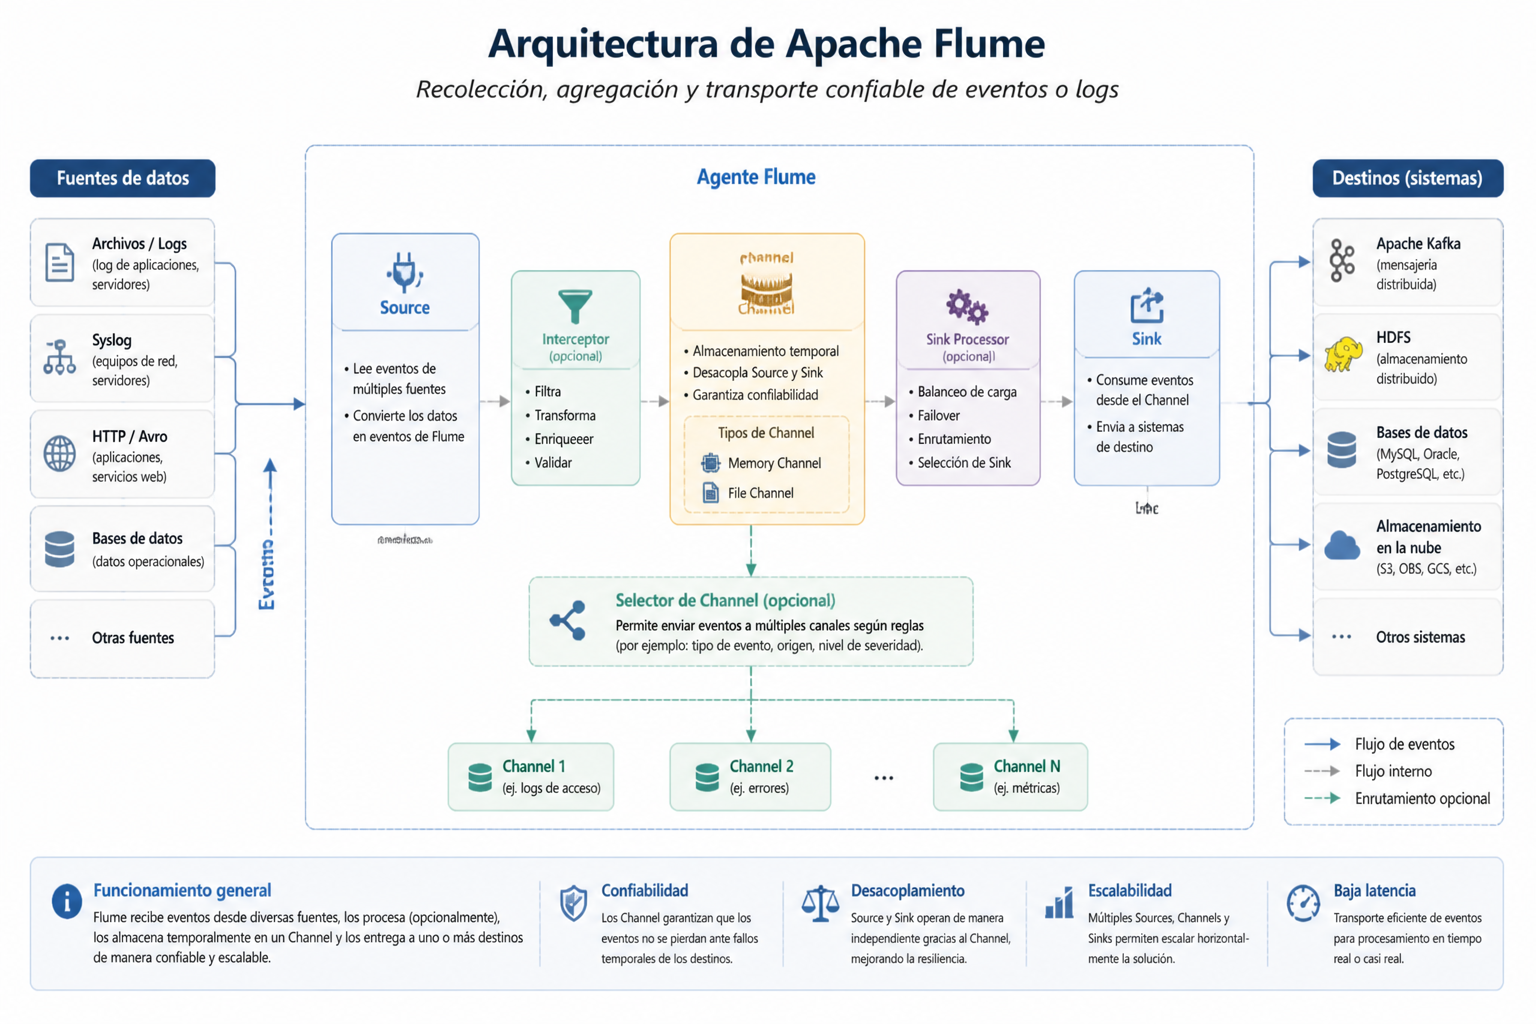
\includegraphics[width=\textwidth]{img/07.png}
\caption{Arquitectura interna de Apache Flume y flujo de eventos entre \textit{source}, \textit{channel} y \textit{sink}}
\label{fig:flume-architecture}
\end{figure}

\subsection{Kafka}

Kafka es una plataforma distribuida de mensajeria y \textit{event streaming}. Organiza los datos en \textit{topics} divididos en particiones, lo que permite paralelismo, persistencia y escalabilidad horizontal. Su utilidad principal dentro de la arquitectura es desacoplar productores y consumidores, absorber variaciones de carga y conservar el historial reciente de eventos para reprocesamiento o multiples consumidores.

Frente a Flume, Kafka no se limita a recolectar eventos: tambien actua como sistema central de distribucion y almacenamiento temporal del flujo. La investigacion enfatiza que su modelo \textit{publish-subscribe}, junto con el manejo de \textit{offsets}, permite que distintos consumidores lean el mismo flujo con independencia entre si. Esto es crucial cuando un mismo evento debe alimentar varios procesos: analitica, auditoria, recomendaciones o persistencia historica.

Ademas, Kafka facilita el desacoplamiento organizacional y tecnico del sistema. Los productores publican sin necesidad de conocer quien procesara los datos despues, mientras que los consumidores pueden evolucionar, escalar o reiniciarse sin alterar directamente a la fuente.

\begin{figure}[h]
\centering
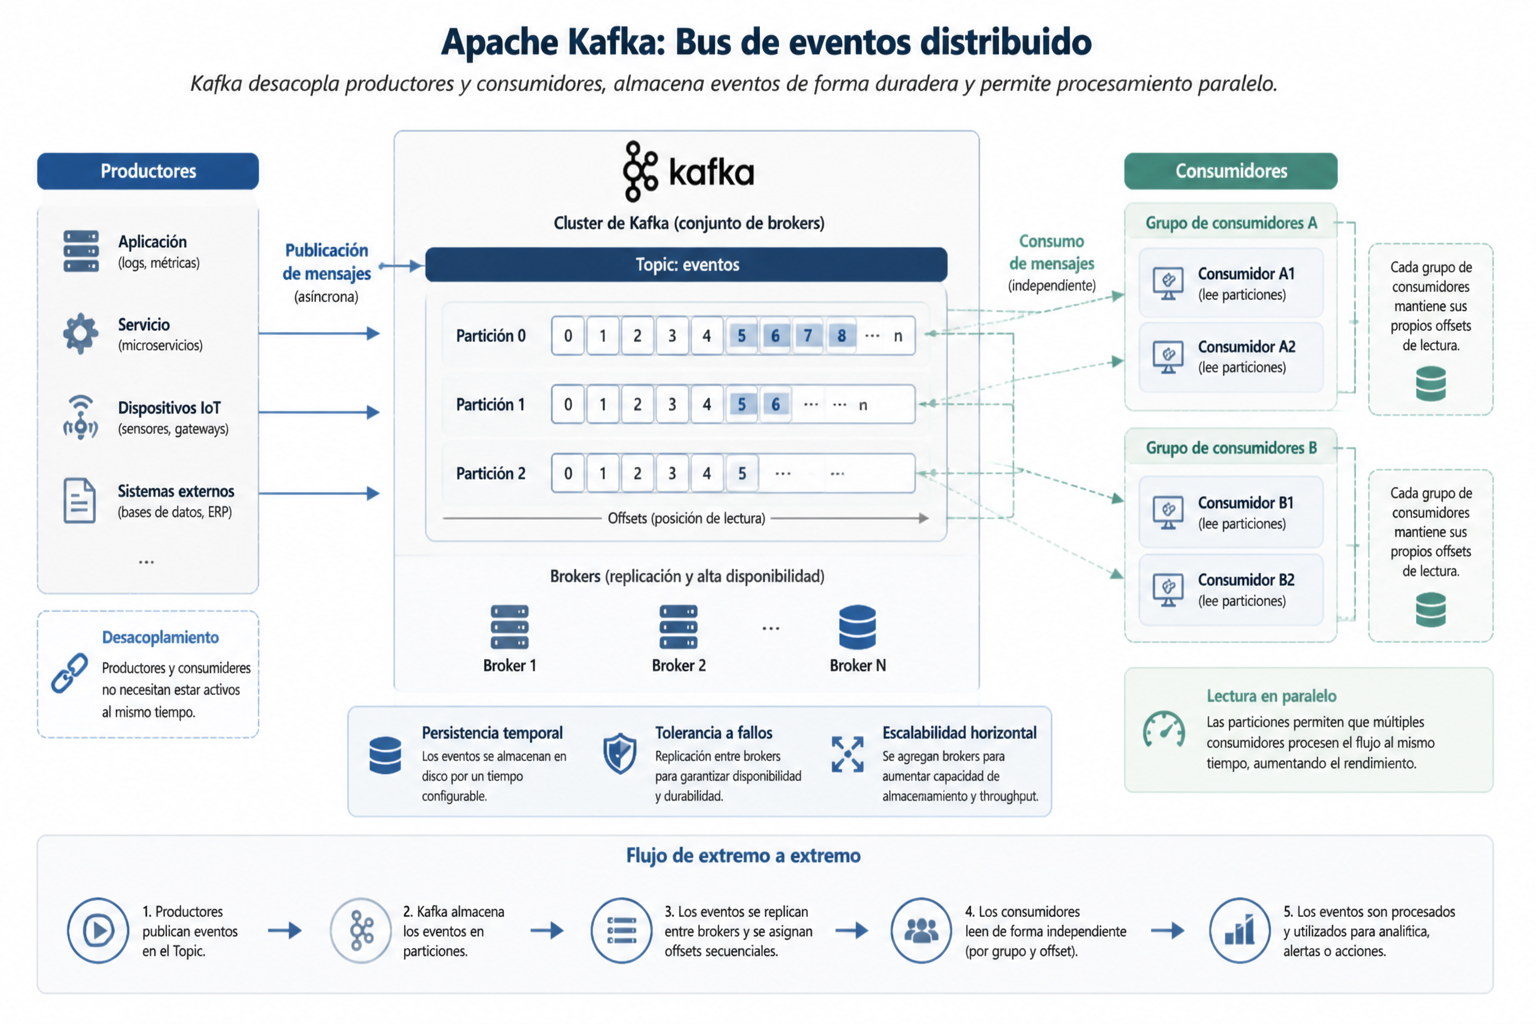
\includegraphics[width=\textwidth]{img/08.png}
\caption{Flujo logico de Kafka con productores, \textit{topics}, particiones y consumidores}
\label{fig:kafka-architecture}
\end{figure}

\subsection{Flink}

Flink es un motor de procesamiento distribuido especialmente fuerte en escenarios de baja latencia, manejo de estado y tiempo de evento. Entre las razones por las que el capitulo lo resalta se encuentran:

\begin{itemize}
  \item procesamiento continuo de flujos acotados y no acotados;
  \item soporte avanzado de ventanas y \textit{watermarks};
  \item tolerancia a fallos basada en estado y \textit{checkpoints};
  \item capacidad de ofrecer semanticas \textit{exactly-once}.
\end{itemize}

Estas propiedades lo vuelven adecuado para fraude, deteccion de anomalias, monitoreo operacional y otras aplicaciones sensibles a la latencia. La investigacion agrega varios puntos relevantes: Flink unifica procesamiento batch y streaming, maneja flujos acotados y no acotados, soporta despliegues sobre YARN, Mesos, Kubernetes o clusters independientes, y fue concebido para operar en escenarios con miles de nodos.

Tambien destaca su manejo explicito de \textit{event time}, sus tipos de ventana y el mecanismo de \textit{checkpoints} con barreras. Por ello, Flink suele considerarse una de las tecnologias mas solidas cuando la correccion temporal y la consistencia del estado son requisitos de primer nivel.

\subsection{Structured Streaming}

Structured Streaming es el motor de streaming de Spark SQL. Su idea central consiste en tratar el flujo como una tabla incremental sobre la que se aplican consultas estructuradas. Esto facilita el uso de operaciones familiares para equipos que ya trabajan con DataFrames o SQL.

La investigacion muestra que este enfoque se apoya en un modelo donde cada consulta produce una tabla de resultados que se actualiza cada vez que ingresan nuevos datos. Tambien resume sus modos de salida mas conocidos: \textit{complete}, \textit{append} y \textit{update}, los cuales determinan si se escribe toda la tabla, solo las filas nuevas o solo las filas modificadas.

Su gran fortaleza es la integracion con el ecosistema Spark, mientras que su compromiso tradicional ha sido una latencia algo mayor que la de motores puramente orientados a evento. Aun asi, resulta muy util para pipelines analiticos, integracion con aprendizaje automatico y laboratorios educativos en Python. Ademas, soporta tiempo de evento, tiempo de procesamiento y manejo de datos tardios mediante \textit{watermarks}, lo que lo vuelve una opcion muy pedagogica para construir practicas sin abandonar el entorno de Spark.

\subsection{Redis}

Redis es una base de datos en memoria orientada a baja latencia. Dentro de una arquitectura de streaming puede utilizarse como cache operativa, almacenamiento temporal de resultados, ranking en tiempo real o soporte de consultas rapidas. No reemplaza al motor de procesamiento, pero complementa el pipeline cuando se necesita una respuesta inmediata hacia aplicaciones o dashboards.

Segun la investigacion, Redis resulta especialmente util en escenarios de \textit{top N}, sesiones, contadores, colas, \textit{pub/sub} y datos con expiracion. Sus estructuras de datos, como cadenas, listas, conjuntos, \textit{hashes} y \textit{sorted sets}, lo convierten en un soporte versatil para resultados de streaming que luego deben ser consultados por una aplicacion con tiempos de respuesta de milisegundos.

\subsection{Comparacion resumida}

\begin{table}[h]
\centering
\caption{Rol principal de las tecnologias del capitulo}
\begin{tabularx}{\textwidth}{>{\RaggedRight\arraybackslash}p{2.5cm}X}
\toprule
\textbf{Tecnologia} & \textbf{Rol principal} \\
\midrule
Flume & Recoleccion y transporte confiable de logs y eventos. \\
Kafka & Bus de eventos, desacoplamiento, persistencia temporal y distribucion. \\
Flink & Procesamiento continuo con bajo retardo, manejo avanzado de estado y tiempo de evento. \\
Structured Streaming & Procesamiento de streams con API estructurada sobre Spark SQL. \\
Redis & Cache y almacenamiento de baja latencia para resultados o consultas rapidas. \\
\bottomrule
\end{tabularx}
\end{table}

\section{Casos de Uso}

\subsection{Fraude con tarjetas}

El caso emblematico del capitulo es la deteccion de fraude bancario. El flujo comienza cuando una transaccion es generada por un canal de pago, como un POS, una banca movil o una pasarela digital. Cada evento incluye datos como identificador de tarjeta, monto, comercio, hora, ubicacion, dispositivo o canal utilizado. Esa informacion se transmite hacia la plataforma de procesamiento en tiempo real, donde primero se recibe, limpia y enriquece con contexto historico y reglas de riesgo.

En esta etapa pueden intervenir varias capas del pipeline. Flume o conectores equivalentes recolectan eventos, Kafka los distribuye y amortigua picos de carga, y un motor como Flink o Structured Streaming analiza la secuencia de transacciones. El procesamiento puede incluir ventanas cortas por tarjeta, correlacion entre eventos recientes, deteccion de montos atipicos, compras simultaneas en regiones incompatibles, cambios bruscos de comportamiento y combinacion con reglas de negocio.

La salida del sistema no es un simple reporte. Dependiendo del resultado del analisis, la operacion puede aprobarse, rechazarse, enviarse a verificacion adicional o incluso congelarse temporalmente la tarjeta. Ademas, el evento puede registrarse en un sistema de auditoria, alimentar un tablero de monitoreo y generar una alerta al cliente o al equipo de riesgo.

\begin{figure}[h]
\centering
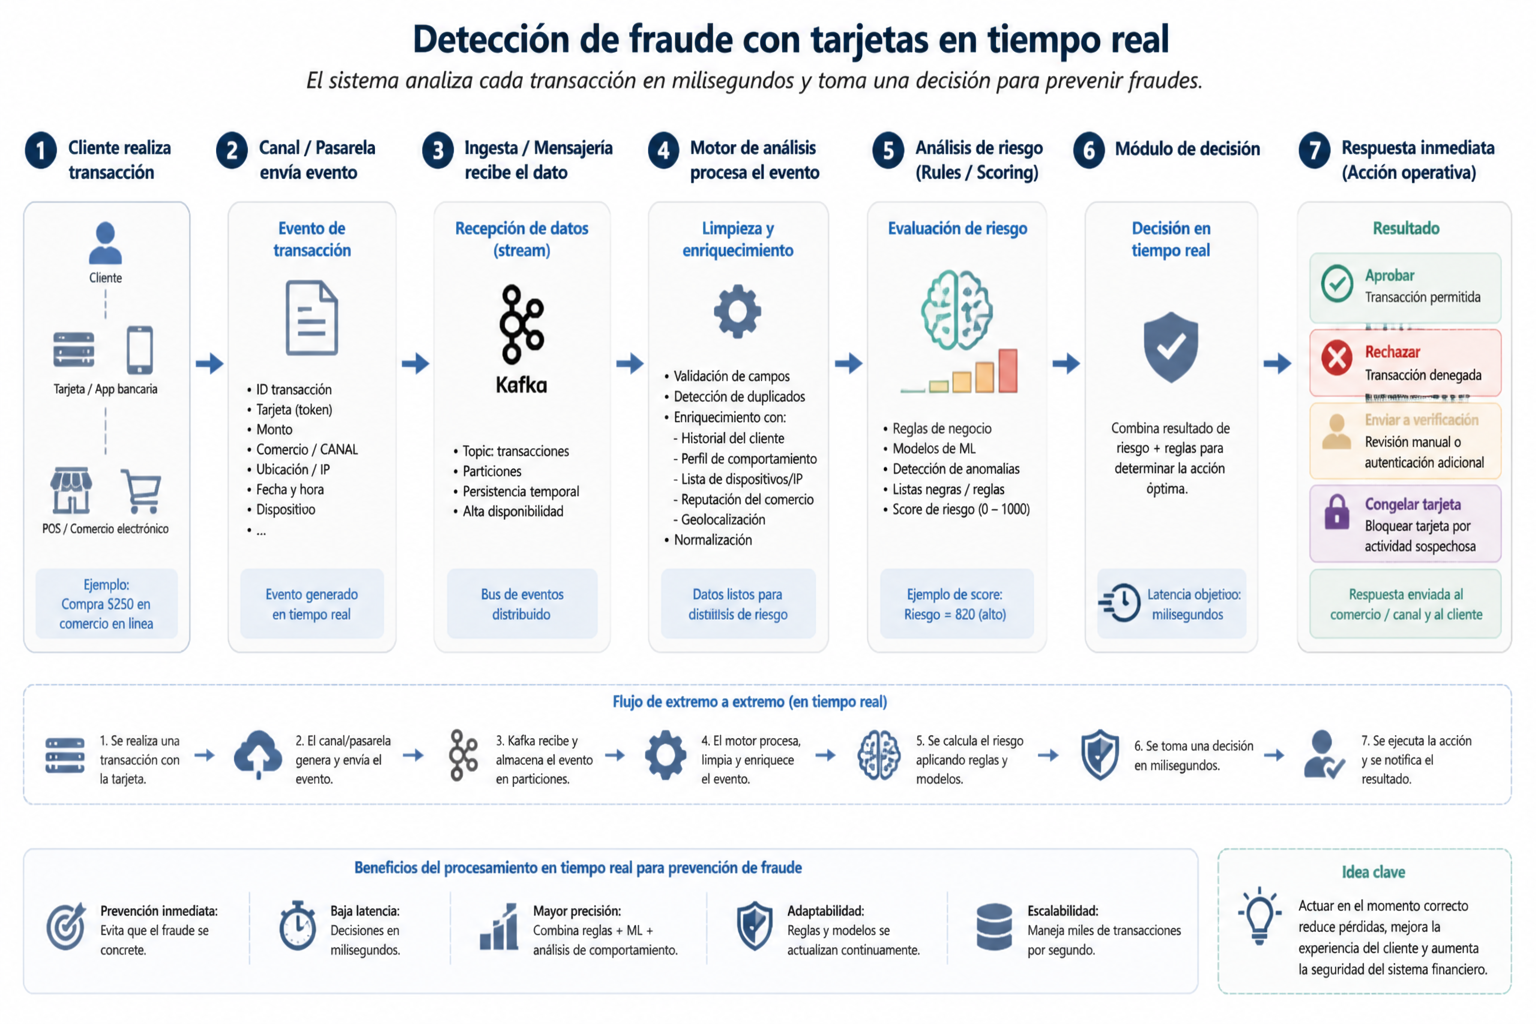
\includegraphics[width=\textwidth]{img/09.png}
\caption{Flujo de deteccion de fraude con tarjetas en una arquitectura de procesamiento en tiempo real}
\label{fig:fraud-streaming-flow}
\end{figure}

La baja latencia es fundamental porque en este escenario el tiempo define la utilidad de la respuesta. Si la deteccion se produce despues de completada la transaccion, la plataforma ya no previene el fraude, sino que solo lo documenta. Por eso este caso expresa con claridad el argumento central del capitulo: el valor del dato disminuye rapidamente y la arquitectura debe responder antes de que la oportunidad de actuar desaparezca.

\subsection{Analitica e-commerce}

Otro caso desarrollado en el material corresponde a una plataforma de comercio electronico que necesita medir ventas y extraer el top 10 de productos en ventanas temporales. Los eventos de entrada pueden ser clics, vistas, productos agregados al carrito, compras efectivas, favoritos o escaneos de catalogo. Cada accion genera un registro con usuario, producto, categoria, marca temporal y tipo de comportamiento.

El procesamiento en tiempo real permite agrupar los eventos por usuario, producto o categoria, calcular metricas recientes y actualizar rankings dinamicos. Por ejemplo, un job de streaming puede medir el monto total vendido cada diez minutos, identificar productos con mayor demanda o construir un perfil instantaneo del comportamiento reciente de un cliente. Redis puede almacenar resultados de baja latencia para dashboards y servicios de recomendacion, mientras Kafka mantiene disponible el flujo para distintos consumidores.

La utilidad de este caso excede la mera estadistica descriptiva. Los resultados pueden alimentar tableros operativos, deteccion de productos tendencia, promociones temporales, ajuste de inventario, segmentacion de clientes y motores de recomendacion. Una recomendacion basada en la accion que el usuario acaba de realizar tiene mucho mas valor comercial que una sugerencia calculada horas despues.

\begin{figure}[h]
\centering
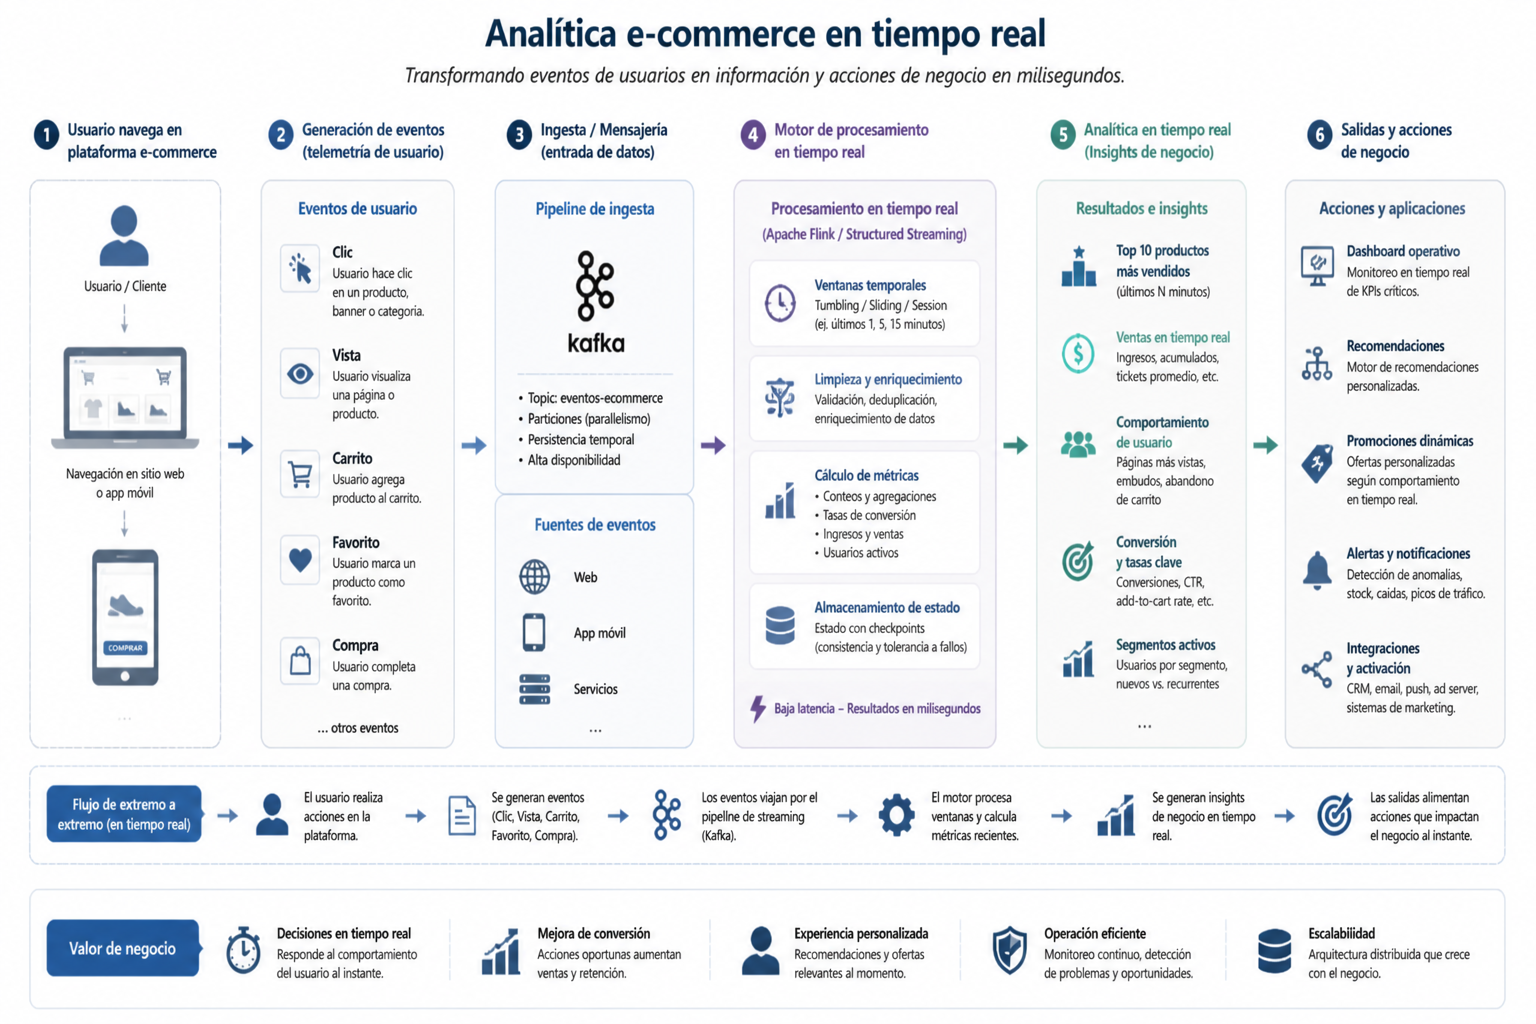
\includegraphics[width=\textwidth]{img/6-2-ecommerce.png}
\caption{Caso de analitica e-commerce en tiempo real basado en eventos de usuario}
\label{fig:ecommerce-streaming}
\end{figure}

Por esa razon, la latencia influye directamente en la experiencia de usuario y en el rendimiento del negocio. Si el sistema identifica a tiempo que un producto esta escalando en ventas, se pueden activar promociones, reorganizar la visibilidad del catalogo o anticipar decisiones logisticas antes de que la oportunidad comercial se pierda.

\subsection{IoT y monitoreo}

En sistemas IoT, los sensores generan telemetria constante sobre temperatura, presion, vibracion, caudal, consumo energetico, posicion o estado de una maquina. Estos eventos suelen llegar con alta frecuencia y, en muchos casos, desde miles de dispositivos distribuidos. El reto no es solo almacenarlos, sino analizarlos de forma continua para detectar situaciones anormales mientras aun es posible intervenir.

Un motor de streaming puede agrupar lecturas por dispositivo o por zona, calcular promedios moviles, desviaciones, maximos, minimos o patrones de variacion, y compararlos con umbrales o modelos predictivos. Si el sistema detecta una temperatura fuera de rango o una vibracion anormal en una turbina, puede disparar alertas de mantenimiento, detener preventivamente una linea o actualizar un tablero en tiempo real.

Este mismo patron se replica en monitoreo de infraestructura digital. Las metricas de CPU, memoria, uso de red y errores de aplicacion se convierten en eventos de entrada que el pipeline correlaciona para anticipar incidentes. En lugar de esperar a que el servicio falle completamente, el sistema identifica deterioros graduales y habilita respuestas tempranas, como escalar recursos, reiniciar componentes o redirigir trafico.

\begin{figure}[h]
\centering
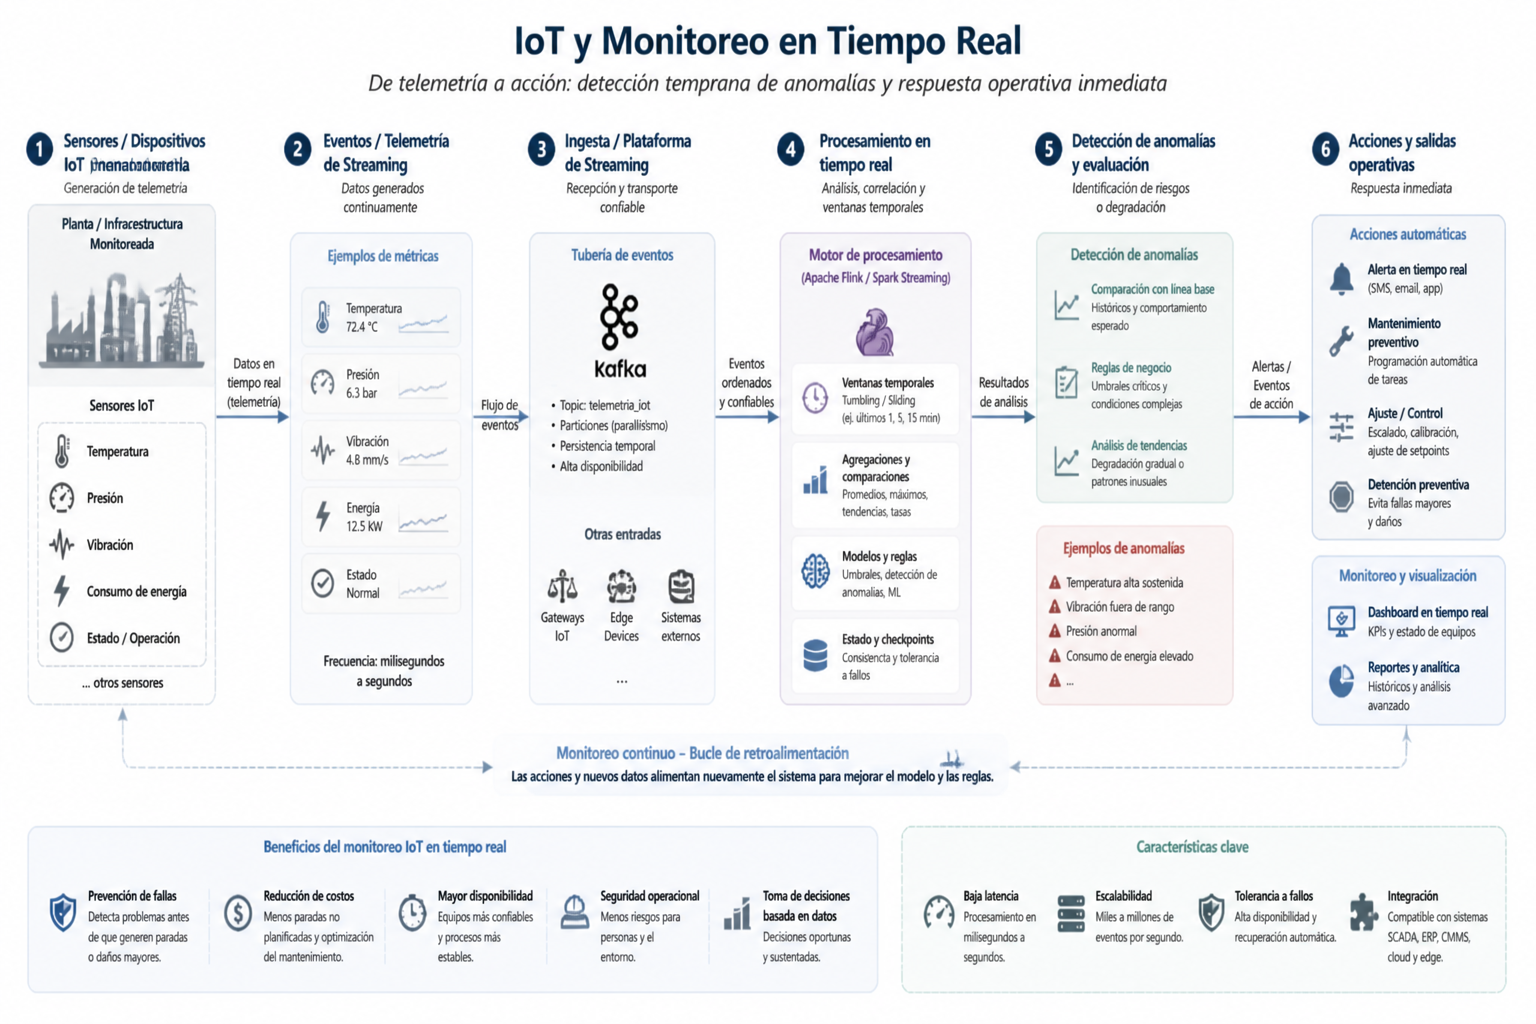
\includegraphics[width=\textwidth]{img/6-3-iot.png}
\caption{Caso de IoT y monitoreo en tiempo real con deteccion de anomalias y respuesta operativa}
\label{fig:iot-monitoring-streaming}
\end{figure}

La importancia de la baja latencia radica en que muchas anomalias evolucionan rapidamente. Detectar una falla inminente algunos segundos antes puede evitar una parada de planta, una perdida economica o una degradacion severa del servicio.

\subsection{Ciberseguridad}

En ciberseguridad, los flujos de logs, intentos de acceso, trafico de red, alertas de firewall, eventos de IDS y registros de autenticacion forman una corriente continua de informacion que debe correlacionarse casi al instante. Un solo evento aislado puede parecer inocuo, pero la secuencia completa puede revelar un ataque en curso.

El procesamiento en tiempo real permite combinar multiples senales: varios intentos fallidos de acceso seguidos de una autenticacion exitosa, conexiones desde ubicaciones inusuales, exploracion de puertos, transferencia anomala de datos o cambios bruscos en patrones de comportamiento. Un motor como Flink puede mantener estado por usuario, IP o servicio, y aplicar ventanas temporales para identificar secuencias sospechosas.

La salida esperada suele ser una accion automatizada o semiautomatica: bloquear una IP, elevar el nivel de riesgo de una sesion, generar una alerta al SOC, registrar evidencia para analisis forense o retroalimentar un SIEM. En entornos modernos, esta capacidad es critica porque una respuesta tardia aumenta la superficie de daño y facilita la exfiltracion de datos.

\begin{figure}[h]
\centering
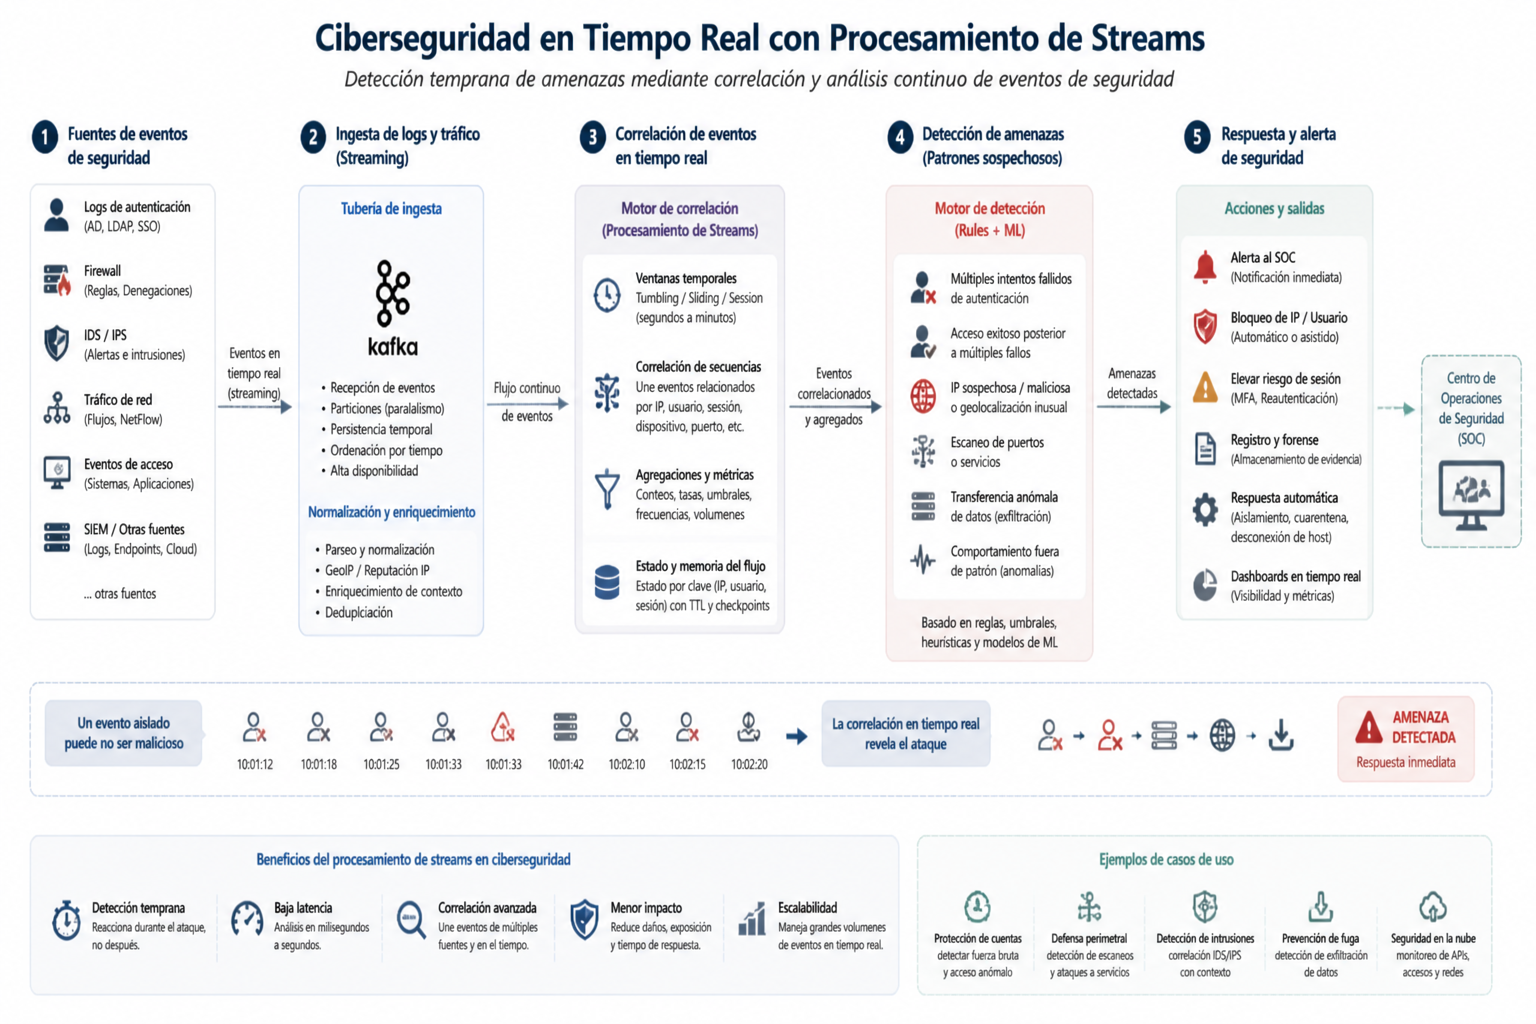
\includegraphics[width=\textwidth]{img/6-4-ciberseguridad.png}
\caption{Caso de ciberseguridad en tiempo real con correlacion de eventos y respuesta inmediata}
\label{fig:cybersecurity-streaming}
\end{figure}

Por ello, la reaccion durante el ataque, y no despues, es lo que justifica la adopcion de pipelines de streaming en centros de operaciones de seguridad.

\subsection{Telecomunicaciones y recomendacion en tiempo real}

El enfoque de \textit{stream processing} tambien resulta especialmente util en telecomunicaciones y en sistemas de recomendacion. En redes de telecomunicacion, los eventos de entrada incluyen registros de llamadas, calidad de señal, logs de estaciones base, uso por celda y alarmas de equipos. El procesamiento por ventanas permite detectar congestion, degradacion de servicio o caidas parciales por region, habilitando ajustes dinamicos de capacidad o intervenciones tecnicas antes de que el problema afecte a un gran numero de usuarios.

En sistemas de recomendacion, ya sea en retail, video, musica o plataformas de contenido, los eventos provienen de navegacion, reproducciones, pausas, clics o compras. El pipeline puede actualizar perfiles de usuario en tiempo real, recalcular rankings y producir sugerencias personalizadas con base en el comportamiento mas reciente. Aqui la salida no siempre es una alerta, sino una accion comercial o de experiencia de usuario: banners dinamicos, listas sugeridas, productos relacionados o promociones contextuales.

En ambos casos, la baja latencia es clave porque la utilidad de la decision depende del momento. Ajustar la red cuando ya ocurrio la saturacion o recomendar contenido cuando el usuario ya abandono la sesion reduce drasticamente el impacto del sistema.

En conjunto, estos casos muestran que el procesamiento en tiempo real no es una tecnologia aislada, sino un paradigma transversal para escenarios donde la secuencia de eventos, el contexto reciente y la velocidad de respuesta determinan el valor final de los datos.

\section{Vigencia y Evolucion del Ecosistema}

Aunque el capitulo 4 sigue siendo conceptualmente vigente, el ecosistema ha evolucionado de forma importante en los ultimos años. La investigacion realizada muestra que las tecnologias principales del capitulo no han perdido relevancia, pero si han cambiado en arquitectura interna, modos de despliegue, integracion con otros sistemas y madurez operativa.

En el caso de Kafka, la evolucion mas visible ha sido la consolidacion de la arquitectura KRaft. Las versiones recientes han eliminado progresivamente la dependencia historica de ZooKeeper y trasladado el control de metadatos al propio cluster. Esto reduce complejidad operativa, simplifica despliegues y mejora la administracion del sistema. Ademas, Kafka ha reforzado sus mecanismos de rebalanceo, su capacidad de escalado y su posicion como plataforma central de eventos para arquitecturas distribuidas.

Flink tambien ha avanzado de manera significativa. La investigacion destaca mejoras en la integracion con SQL, conectores mas ricos, despliegues sobre Kubernetes y una orientacion creciente hacia arquitecturas de tipo \textit{streaming lakehouse}. A esto se suma la maduracion de sus capacidades de procesamiento de estado, optimizacion sobre RocksDB y adopcion en entornos donde la consistencia temporal y la semantica \textit{exactly-once} son decisivas. En otras palabras, Flink no solo sigue vigente, sino que se ha fortalecido como una plataforma especializada para procesamiento de eventos complejos.

Por su parte, Structured Streaming ha extendido sus capacidades dentro del ecosistema Spark. Aunque tradicionalmente se ha apoyado en un modelo de micro-batches, la investigacion muestra que el entorno Spark 3.x ha reforzado modos de procesamiento mas cercanos al tiempo real y una integracion cada vez mayor con Delta Lake, tablas ACID y pipelines de aprendizaje automatico. Esto lo mantiene como una alternativa especialmente atractiva para equipos que ya trabajan con DataFrames, SQL y herramientas analiticas del ecosistema Spark.

Otra linea de evolucion importante es la diversificacion del ecosistema de ingesta y mensajeria. Ademas de Flume y Kafka, hoy existen soluciones como Apache Pulsar, Amazon Kinesis o Google Pub/Sub, que responden a necesidades de multi-tenencia, administracion en la nube o escalado administrado. Esto significa que la arquitectura presentada en el capitulo puede mantenerse, pero las piezas concretas pueden variar segun el contexto tecnico y organizacional.

La investigacion tambien incorpora una discusion sobre patrones arquitectonicos modernos. En particular, se menciona el patron Kappa como alternativa a arquitecturas donde se separan capa batch y capa streaming. La idea central del patron Kappa es reutilizar una unica logica de procesamiento sobre un flujo persistido, reduciendo duplicacion de codigo y simplificando el mantenimiento. No obstante, en algunos escenarios siguen siendo validas arquitecturas hibridas que combinan velocidad en tiempo real con correcciones posteriores sobre datos historicos.

En consecuencia, el valor actual del capitulo 4 no radica en ofrecer una fotografia definitiva del estado del arte, sino en proporcionar una base conceptual robusta. Sus principios sobre latencia, \textit{throughput}, estado, ventanas, tolerancia a fallos y desacoplamiento continúan siendo plenamente utiles. Lo que cambia es la implementacion concreta de esos principios en herramientas mas maduras, despliegues cloud-native y patrones arquitectonicos mas refinados.

Esto no invalida el contenido del libro. Por el contrario, confirma que sus fundamentos siguen siendo utiles, pero que conviene complementarlos con documentacion actual cuando se diseña un laboratorio o una implementacion real.

\section{Implicancias para el Laboratorio}

Desde una perspectiva pedagogica, el tema del capitulo se presta muy bien para un laboratorio orientado a un caso de negocio concreto. En esta exposicion se implemento una demostracion local basada en deteccion de fraude con tarjetas, porque este escenario permite reunir en un solo flujo los conceptos de latencia, tiempo de evento, ventanas, estado, \textit{watermarks}, duplicados y decisiones operativas.

\subsection{Objetivo del laboratorio}

El laboratorio busca mostrar de forma verificable como funciona un pipeline de \textit{stream processing} cuando los datos llegan continuamente, pueden llegar fuera de orden y deben convertirse en una accion inmediata. En lugar de limitarse a leer un archivo y calcular un conteo, la implementacion se centro en reproducir la logica del capitulo: una fuente produce transacciones, un broker intermedio desacopla la llegada de eventos, un motor de procesamiento conserva estado por tarjeta y un \textit{sink} emite decisiones.

\subsection{Flujo implementado}

La arquitectura del laboratorio puede resumirse mediante el flujo de la Figura~\ref{fig:lab-flow}. Aunque no se levanta un cluster real de Kafka o Flink en esta version, la demostracion conserva la misma estructura conceptual del capitulo.

\begin{figure}[h]
\centering
\begin{tikzpicture}[node distance=0.75cm]
  \node[box] (src) {Fuente de\\transacciones};
  \node[box, right=of src] (broker) {Broker\\simulado};
  \node[box, right=of broker] (proc) {Motor de\\streaming};
  \node[box, right=of proc] (sink) {Sink de\\decisiones};
  \node[smallbox, below=of proc] (ckpt) {Checkpoints};
  \node[smallbox, above=of sink] (dash) {Dashboard\\web};

  \draw[line] (src) -- (broker);
  \draw[line] (broker) -- (proc);
  \draw[line] (proc) -- (sink);
  \draw[line] (proc) -- (ckpt);
  \draw[line] (sink) -- (dash);
\end{tikzpicture}
\caption{Flujo conceptual del laboratorio de fraude en tiempo real}
\label{fig:lab-flow}
\end{figure}

La fuente esta formada por un conjunto de eventos JSONL donde cada transaccion contiene \textit{event\_id}, tarjeta, comercio, monto, pais, \textit{event time} y \textit{arrival time}. El broker simulado preserva la idea de una cola intermedia que desacopla produccion y consumo. Sobre ese flujo, el motor de streaming procesa por orden de llegada, pero aplica las reglas usando tiempo de evento. Finalmente, el \textit{sink} produce decisiones como aprobar, revisar, bloquear, auditar por tardanza o ignorar duplicados.

\subsection{Conceptos demostrados}

La implementacion del laboratorio permite observar de manera directa los siguientes conceptos:

\begin{itemize}
  \item \textbf{Event time vs. processing time}: los eventos se ordenan por \textit{arrival time}, pero las reglas operan con \textit{event time}, lo que permite explicar por que la hora real del suceso y la hora de procesamiento no siempre coinciden.
  \item \textbf{Ventanas}: el estado por tarjeta se mantiene dentro de una ventana temporal configurable para detectar concentraciones de gasto y frecuencia anomala.
  \item \textbf{Estado}: el motor conserva informacion reciente por tarjeta, como ultimo pais observado, cantidad de transacciones en ventana y monto acumulado.
  \item \textbf{Watermarks}: el sistema avanza un \textit{watermark} a partir del maximo \textit{event time} observado y marca como tardios los eventos que llegan demasiado atras respecto a esa referencia.
  \item \textbf{Deduplicacion}: si un mismo \textit{event\_id} aparece dos veces, el segundo evento se ignora para ilustrar comportamiento idempotente y una aproximacion pedagogica a semanticas de entrega robustas.
  \item \textbf{Checkpoints}: cada cierto numero de eventos se guarda un snapshot del estado para explicar la idea de recuperacion y continuidad del procesamiento.
\end{itemize}

\subsection{Reglas y decisiones del motor}

Las reglas implementadas son deliberadamente sencillas, pero suficientes para mostrar la logica de negocio en tiempo real:

\begin{itemize}
  \item \textbf{APROBAR}: no se detecta patron sospechoso.
  \item \textbf{REVISAR}: el monto individual es muy alto o se observa un cambio de pais en un lapso corto.
  \item \textbf{BLOQUEAR}: existe alta frecuencia de transacciones junto con un monto acumulado elevado dentro de la ventana.
  \item \textbf{AUDITAR\_TARDE}: el evento llega demasiado tarde respecto al \textit{watermark}.
  \item \textbf{IGNORAR\_DUPLICADO}: el \textit{event\_id} ya fue procesado previamente.
\end{itemize}

Estas decisiones permiten relacionar el laboratorio con el caso de fraude descrito en el capitulo: la arquitectura no solo observa el dato, sino que traduce el flujo en una accion operativa.

\subsection{Visualizacion y explicacion del flujo}

Ademas de la salida por consola, el laboratorio incorpora un dashboard web local que permite mostrar el pipeline de forma visual durante la exposicion. Esta interfaz presenta cuatro etapas: fuente, broker, procesador y \textit{sink}. Tambien exhibe el evento actual, la profundidad de la cola, el \textit{watermark}, el resumen de decisiones y una tabla de eventos recientes. De este modo, el estudiante no solo afirma que existe un flujo continuo, sino que puede verlo y explicarlo en tiempo real.

\subsection{Alcance tecnico y valor pedagogico}

Por restricciones del entorno de trabajo, esta version prioriza una implementacion local estable en Python sobre un despliegue completo con Kafka, Flink o Spark. Sin embargo, la demostracion conserva los principios fundamentales del capitulo y por ello resulta adecuada para fines academicos. Su principal valor pedagogico es que transforma teoria en observacion: el estudiante puede seguir el recorrido del evento, identificar un caso tardio, observar la deduplicacion y verificar como cambia la decision del sistema conforme se acumula contexto reciente.

En consecuencia, el laboratorio no debe verse como una simplificacion trivial, sino como una maqueta funcional de los elementos conceptuales del procesamiento de flujos en tiempo real a gran escala. Tambien deja abierta una ruta de evolucion futura hacia una arquitectura mas cercana al stack del capitulo, por ejemplo mediante productor Python, Kafka real, PySpark Structured Streaming o PyFlink y salida a Redis o a un dashboard conectado en vivo.

\section{Conclusiones}

El procesamiento de flujos de datos en tiempo real a gran escala responde a una necesidad central de los sistemas modernos: actuar mientras el dato aun conserva valor operativo. A diferencia del enfoque \textit{batch}, el \textit{stream processing} exige computo continuo, control temporal, manejo de estado y recuperacion consistente frente a fallos.

El capitulo 4 de \textit{huawei-2022.pdf} ofrece una introduccion aplicada y coherente a este problema mediante una arquitectura basada en Flume, Kafka, Flink, Structured Streaming y Redis. Cada componente cumple una funcion especifica dentro del pipeline, desde la ingesta hasta la accion final.

La investigacion complementaria muestra que el ecosistema ha seguido madurando, pero sin alterar sus principios fundamentales. Por ello, la combinacion entre el contenido del libro y las practicas actuales permite construir una monografia solida, una presentacion clara y un laboratorio tecnicamente relevante para el curso.

\newpage

\begin{thebibliography}{99}

\bibitem{huawei2022}
Huawei Technologies Co., Ltd., \textit{HCIP Big Data Developer V2.0 Training Material}, 2022.

\bibitem{kafka-docs}
Apache Kafka, ``Documentation,'' \url{https://kafka.apache.org/documentation/}, consultado en mayo de 2026.

\bibitem{kafka40}
Apache Kafka, ``Apache Kafka 4.0 Announcement,'' \url{https://kafka.apache.org/40/}, consultado en mayo de 2026.

\bibitem{flink-docs}
Apache Flink, ``Flink Documentation,'' \url{https://nightlies.apache.org/flink/}, consultado en mayo de 2026.

\bibitem{spark-ss}
Apache Spark, ``Structured Streaming Programming Guide,'' \url{https://spark.apache.org/docs/latest/structured-streaming-programming-guide.html}, consultado en mayo de 2026.

\bibitem{flume-docs}
Apache Flume, ``Flume User Guide,'' \url{https://flume.apache.org/FlumeUserGuide.html}, consultado en mayo de 2026.

\bibitem{redis-docs}
Redis, ``Redis Documentation,'' \url{https://redis.io/docs/}, consultado en mayo de 2026.

\bibitem{conduktor-flink}
Conduktor, ``What is Apache Flink?,'' \url{https://www.conduktor.io/}, consultado en mayo de 2026.

\bibitem{research-stream}
T. Akidau et al., ``The Dataflow Model: A Practical Approach to Balancing Correctness, Latency, and Cost in Massive-Scale, Unbounded, Out-of-Order Data Processing,'' \textit{Proceedings of the VLDB Endowment}, vol. 8, no. 12, 2015.

\end{thebibliography}

\end{document}
